\section{Architecture Overview}

\begin{figure}[H] \centering 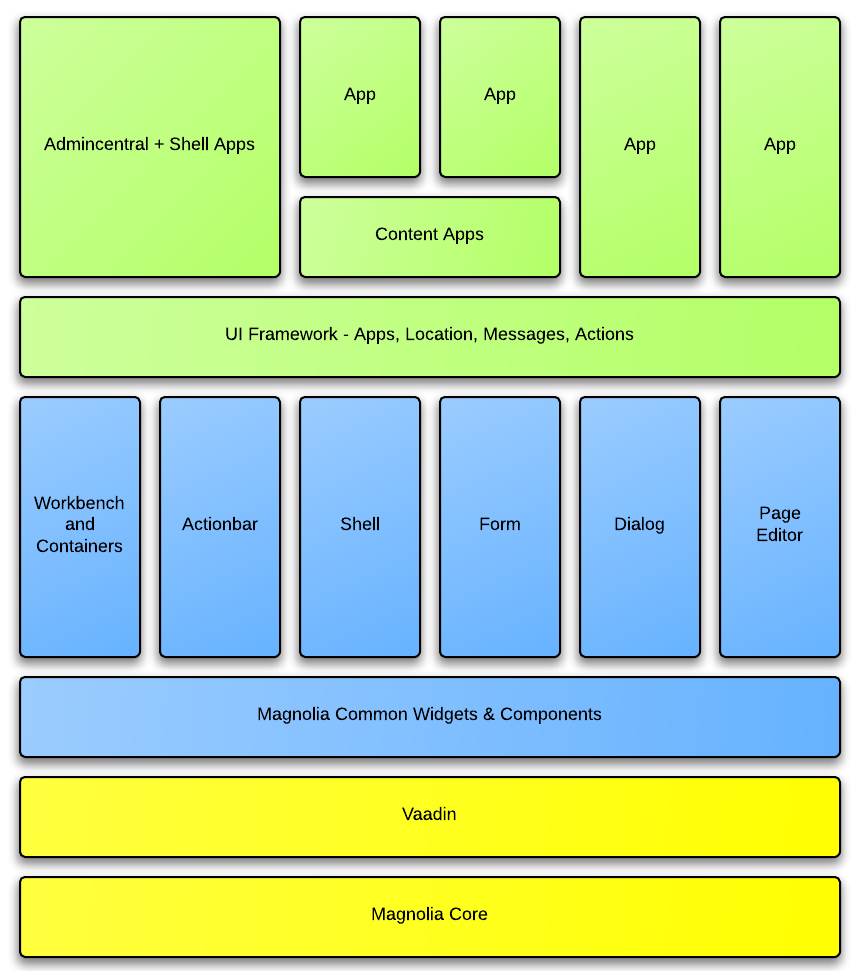
\includegraphics[width=\textwidth]{architecture_layers.png}
	\caption{High-level architecture overview}
	\label{fig:architecture_overview}
\end{figure}

Firgure ~\ref{fig:architecture_overview} displays the structure of the project
architecture. The main goal of a such architecture design is to provide a set of loosely
coupled components and interfaces. The block structure means that every block is
a separate Magnolia CMS module which encapsulates a logical part of the system.
The firgure ~\ref{fig:architecture_overview} also describes the dependency
hierarchy of the project: the parts of the system can only depend on the blocks
that belong to the layer that resides below in the diagram. This means that most
low-level tiers of the architecture are core Magnolia API and plain Vaadin
components and interfaces, whereas the top-level parts are apps - parts of the
system actually visible to an end-user. Apps can re-use any API and frameworks
present in the system. Let us briefly discuss the features of all the layes of
the architecture.

\subsection{Magnolia Core API and Vaadin} 
  The main two frameworks used in the system
  provide a low-level foundation of Magnolia AdminCentral module. Magnolia Core
  API enables interfaces and utilities for accessing JCR, dependency injection
  functionality, tools for localization etc. Vaadin serves as a platform for the
  Magnolia AdminCentral web-application and abstract building blocks
  (Components) for moe specific parts of teh system.
\subsection{Magnolia Common Widgets and Components} 
  This layer of the system aggregates the essential re-usable components built on top of the core
  frameworks. Such components include, for instance, the page editor - the
  What-You-See-Is-What-You-Get (WYSIWYG) utility for modifying the website
  pages. Common Components layer also includes the data management structures
  such as JCRContainer.
\subsection{UIFramework} 
  UIFramework layer provides the foundation for the apps,
  such as base classes and interfaces, action-execution mechanisms and message
  exchange infrastructure. UIFramework also contains the fundamental
  communication framework for the entire AdminCentral web application, which is
  called Location Framework.
\subsection{AdminCentral and apps}
  Finally, the top-most architecture layer is reserved for apps and AdminCentral
  web application. An app represents a logically and functionally consistent
  unit that allows for conducting certain operations on the contnet and/or the
  essentail workflow utilities.

In the current chapter we will mostly discuss the concept of the UIFramework in
detail. The importance of UIFramewor cannot be overestimated because it is a connection
point between the core API's and comonents and the apps. We will pay additional
attention to the app-framework as well. The following chapter
(\ref{implementation}) will highlight the implementation details of the most
crucial components from the common widgets layer.
